\newpage
\section{Sleep Well}
\subsection{Data understanding and preprocessing}

Since labels are integers, we can use \texttt{np.bincount()} to easily count
them:
\begin{minted}[frame=none]{python}
y_train_counts = np.bincount(y_train)
y_train_freqs  = y_train_counts / y_train_counts.sum()
\end{minted}
\emph{See lines 48-51 of }\texttt{code/q4/run.py}.

The frequencies are plotted and shown in \Cref{fig:class_freqs}. I also show the
test data class frequencies, as it may be relevant later to be able to compare
class balance between the training and testing sets.

\begin{figure}[H]
  \centering
  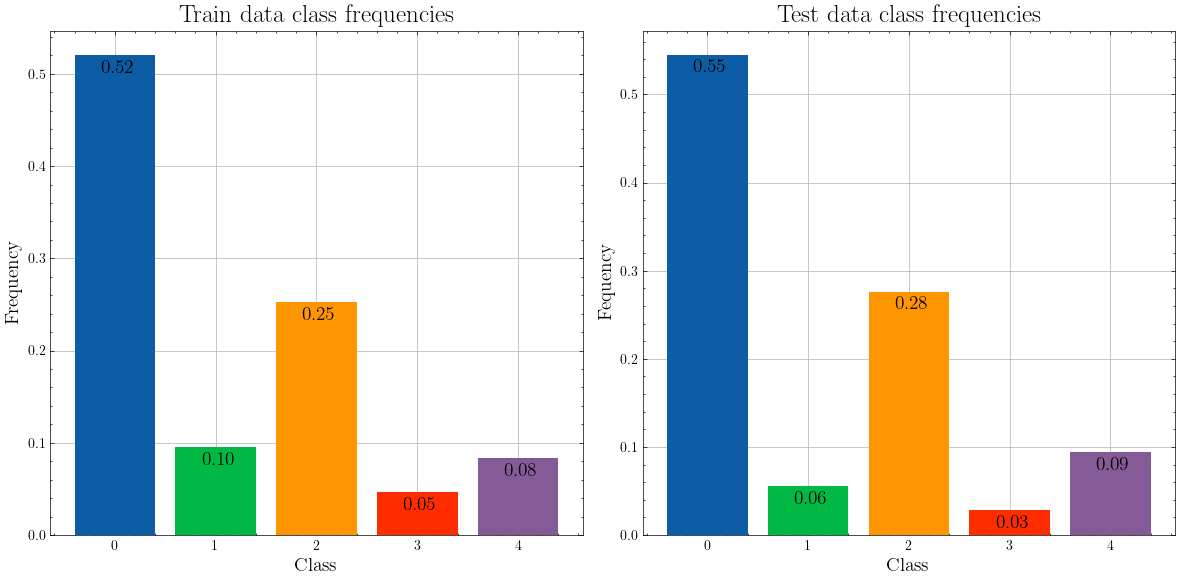
\includegraphics[width=\textwidth]{figures/q4_class_freqs.png}
  \vspace{-0.5cm}
  \caption{\footnotesize \textit{Class frequencies for the sleep stage data.}}
  \label{fig:class_freqs}
\end{figure}

\subsection{Principal component analysis}

I write my own PCA implementation (see lines 7-40 of
attached\texttt{code/q4/my\_stuff.py}), which can be found in the class. In lines 87-90 of
\texttt{code/q4/run.py}, I perform the PCA, compute explained variance, and
project the training dataset onto the first two PC's as such:

\begin{minted}[frame=none]{python}
PCA = my_stuff.MyPCA()
PCA.fit(X_train)
first_above_90 = (PCA.exp_var.cumsum() >= 0.9).argmax() + 1
proj1, proj2, *_ = PCA.project(X_train, n_components = 2).T
\end{minted}

\Cref{fig:eigenspectrum} shows the eigenspectrum for the 16 PC's in the training
data.

\begin{figure}[H]
  \centering
  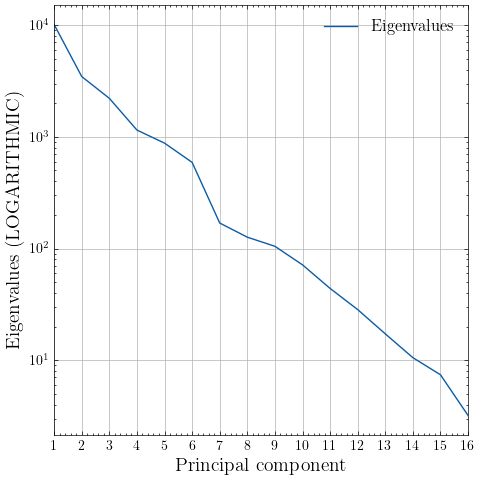
\includegraphics[width=\textwidth]{figures/q4_eigenspectrum.png}
  \vspace{-0.5cm}
  \caption{\footnotesize \textit{Eigenspectrum of the sleep stage training
  data.}}
  \label{fig:eigenspectrum}
\end{figure}

\subsubsection{Explained variance}

To explain 90\% of training data variance requires \textbf{at least 5 PC's}, and
the first 5 PC's explain \textbf{93.8\%} of variance.

\subsubsection{Projecting training data onto PC's}

Next, I project the training data onto the first two PC's and plot the data
points in colors corresponding to their class labels in
\Cref{fig:pca_projection}.

\begin{figure}[H]
  \centering
  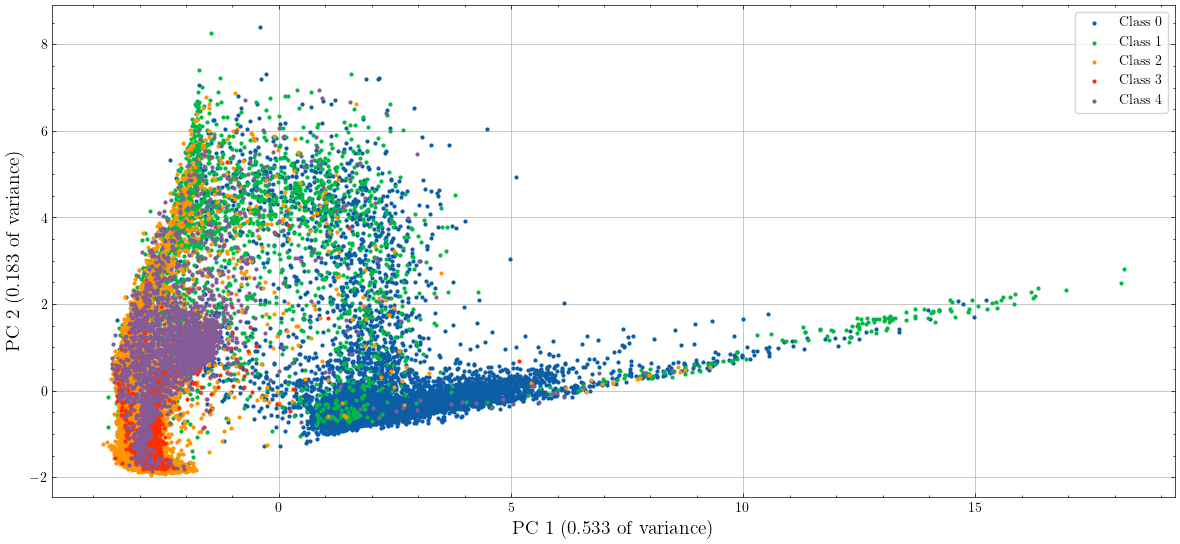
\includegraphics[width=\textwidth]{figures/q4_pca_projection.png}
  \vspace{-0.5cm}
  \caption{\footnotesize \textit{Projection of the sleep stage training data
  onto the first two PC's.}}
  \label{fig:pca_projection}
\end{figure}

\subsection{Clustering}

I use my own implementation of \texttt{k-means} clustering, which supports
\texttt{k-means++} cluster initialization (see \texttt{MyKMeans} in the attached
\texttt{code/q4/my\_stuff.py}) to perform the clustering.

Below \Cref{fig:clustered_pca_project} shows the clustered training data
projected onto the first two PC's, with cluster centroids highlighted with
large, colored circles.

\begin{figure}[H]
  \centering
  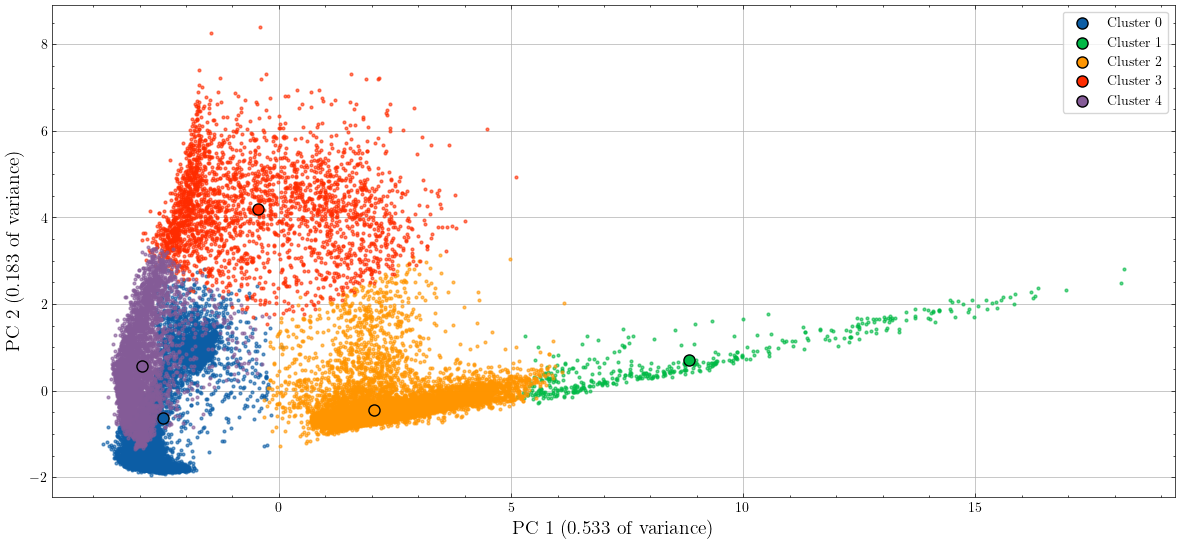
\includegraphics[width=\textwidth]{figures/q4_5-means_pca_projection.png}
  \vspace{-0.5cm}
  \caption{\footnotesize \textit{Projection of \textbf{clustered} sleep stage
  training data onto the first two PC's.}}
  \label{fig:clustered_pca_project}
\end{figure}

As expected, the data does not appear perfectly separated in two dimensions.
This is perhaps in part explained by the fact that the two first PC's explain
only 71.6\% of variance -- aside from this, a pretty good clustering.

\subsection{Classification}
\label{sec:classification}

Before I start work on the three classification methods, I split the training
data up into 70\% training and 30\% validation data (using stratified splitting
to preserve class balance), which will be used during model design in
\cref{sec:mlr} and \cref{sec:rf}.

Please see lines 29-43 of \texttt{code/q4/run.py}.

\subsubsection{Multinomial logistic regression}
\label{sec:mlr}

I am going to use \texttt{Pytorch} to perform the logistic regression.

I design a very simple multi-classification network consisting of an FC layer
with 16 inputs, 32 outputs, and ELU activation; a batch normalization layer; and
an output FC layer with 32 inputs, 5 outputs (one for each label), and softmax
activation:

\begin{minted}{python}
input_dim   = X_train.shape[1]
fc1_units   = 32
num_classes = len(np.unique(y_train))

model = nn.Sequential(
    nn.Linear(input_dim, fc1_units),
    nn.ELU(),
    nn.BatchNorm1d(fc1_units),
    nn.Linear(fc1_units, num_classes),
    nn.Softmax(dim = 1)
)
\end{minted}

I use an Adam optimizer with a learning rate of $0.0001$ and a categorical
cross-entropy loss function, which is suitable for single-label multi-class
classification problems.

This can all be found in lines 187-205 of \texttt{code/q4/run.py}.

I use 2000 epochs in training, and I go through a total of 7 training iterations
of the model design before I settle on the model design described above.

Finally, I train the model on the entire training data and compute zero-one loss
on the testing data. Please see \cref{sec:classifier_results} for the results.


\subsubsection{Random forest classification}
\label{sec:rf}

I use \texttt{sklearn.ensemble.RFClassifier} to build and train the random
forest classifier.

I initially build a forest with no maximum depth and no maximum on the number of
features considered at each tree node (\texttt{max\_depth} and
\texttt{max\_features}, respectively), which obtained a decent
\textbf{validation} loss of about 0.11, but a very suspicious training loss of
0.0, for all three forest sizes.

Very low training loss is not unusual for random forests, and is not
\textit{necessarily} a sign of overfitting -- however, I found better validation
loss scores by reducing the maximum tree depth to 12 and the maximum number of
considered at each internal node to 8.

In addition, the forest was built using Gini impurities and with sample
bootstrapping enabled, since the training data set is large.

\begin{minted}{python}
RFC = RFClassifier(n_estimators = num_trees,
                   criterion = "gini", # use Gini impurities.
                   bootstrap = True,   # use bootstrap samples.

                   max_depth = 12,     # found via manual search.
                   max_features = 8,   # found via manual search.

                   n_jobs = -1,        # might aswell parallelize.
                   random_state = 2,   # for reproducibility.
                  )
\end{minted}

Finally, the model is run on the entire training and testing data -- the
results will be discussed in \cref{sec:classifier_results}.

\newpage
\subsubsection{k-NN classification}
\label{sec:knn}

I implement my own \texttt{k-NN} classifier in the attached
\texttt{code/q4/my\_stuff.py}. The implementation is quite straight-forward, but
uses quickselection to find the \texttt{k} smallest distances in $O(n)$ time
rather than $O(n\, \text{log}\, n)$ as with regular sorting. Below is a snippet
of the interesting parts of my implementation:

\begin{minted}{python}
class MyKNN():
    ...
    def __knn_single_point_single_k(X_train, y_train, x, k):
        dists     = ((X_train - x) ** 2).sum(1)            # dists from x to each train point.
        kn_labels = y_train[np.argpartition(dists, k)[:k]] # sort dists and extract labels.
        return np.bincount(kn_labels).argmax()             # count labels; do majority vote.

    def __knn_many_points_single_k(X_train, y_train, X_test, k):
        return np.array(
            [MyKNN.__knn_single_point_single_k(X_train, y_train, x, k)
             for x in X_test])

    def predict(self, X_test):
        ... # check that model is fitted.
        return MyKNN.__knn_many_points_single_k(self.X_train, self.y_train,
                                                X_test, self.k)
    ...
\end{minted}

\paragraph{Cross-validated parameter search}~

To perform the cross-validated parameter search for the optimal value of
\texttt{k} for the training data, I write a simple grid search, which can be run
on a (one-dimensional) grid of possible \texttt{k} values. The grid search uses
stratified k-fold splitting to generate validation sets\footnote{Note that the
validation sets used here are based on k-fold splits of the \textit{full}
training data, not the training data defined in \cref{sec:classification}.}, and
picks the \texttt{k} which on average produced the smallest losses. This is in
lines 184-218 of \texttt{code/q4/my\_stuff.py}.


The grid search is executed as such: First, the search space is pruned by
searching \texttt{k} $ = 2^i - 1$ for $i \in \{2..13\}$, ie. the set $K_0 = \{3,
7, 15, 31, 63, ..., 8191\}$. The max value of in $K$ is chosen as such because
it is roughly 1/4 of the training data ($n = 33724$), and the optimal value of
$k$ is \textit{very unlikely} to be found in higher ranges.

Next, when the pruning has found an initial value for \texttt{k} in $K$, the
grid search is repeated over all odd numbers between the previous and next value
in $K$. While this is by no means guaranteed to find the optimal \texttt{k}, it
is a good approximation since searching the entire space of possible \texttt{k}
values is not feasible when $n$ is 33724.

The result of pruning is that \texttt{k} $= 63$ is optimal amongst $K_0$; then,
I repeat the search on the grid $K_1 = \{33, 35, \dots\, 125, 127\}$, and find
the overall best \texttt{k} to be \texttt{k} $= 51$.

To reproduce, run \texttt{python code/q4/run.py --do\_gridsearch\_k}.

Using the optimal \texttt{k}, I run \texttt{51-NN} classification on the test
set using the full training data. The results will be presented in
\cref{sec:classifier_results}.

\subsection{Results and discussion}
\label{sec:classifier_results}

\Cref{table:classifier_results} shows the training/testing loss for all 5
classifiers.

\begin{table}[H] \centering
  \begin{tabular}{|l|l|l|}
    \hline
\textbf{Model}                    & \textbf{Training 0-1 loss} & \textbf{Testing 0-1 loss}\\\hline\hline
Multinomial logreg neural network & 0.1570                     & 0.0955  \\\hline
RF (\texttt{num\_trees} = 50)     & 0.0596                     & 0.1099  \\\hline
RF (\texttt{num\_trees} = 100)    & 0.0585                     & 0.1089  \\\hline
RF (\texttt{num\_trees} = 200)    & 0.0581                     & 0.1030  \\\hline
k-NN classifier (k = 51)          & 0.1449                     & 0.0978  \\\hline
\end{tabular}
  \caption{\textit{Classifier training/testing performance comparison (task 4.4).}}
  \label{table:classifier_results}
\end{table}

All five classifiers perform quite well on the testing set, with very similar
loss scores (mean = 0.103, variance = 3.314e-05).

However, it is interesting to note that the logreg network and \texttt{k-NN}
classifier each achieved smaller test loss than training loss. This is sometimes
a sign of underfitting, but in this case I would argue that it is more likely
due to an improper training/test split from the original data. This is
\textit{in some small part} evidenced by the class frequencies in the testing
data (see \cref{fig:class_freqs}), which shows a \textit{slight} class imbalance
between the training and testing data -- but this is only a hunch and should be
further investigated before a conclusion is drawn.

% \TODO{
% logreg network
% trains very fast. also best test score. model {design} took the longest out of the
% three methods, but training was efficient:. VERY fast inference!!!
% }
%
% \TODO{this. training was EASY and quick. a note about how it is pretty easy to
% get training loss of 0.0 using random forests, but this very surely results in
% overfitting. I avoid overfitting by setting max\_depth = 12 and max\_features = 8
% to limit the height of the trees and the number of features considered at each
% internal tree nodes. also, inference is pretty quick, though not as quick as
% network.}
% \TODO{this.
% >> KNN
% Inference on training points took VERY long time; okay for test points, since
% there were less of them, but still took longer than the other two methods.
% advantage is no training time, since it is effectively "learning" during
% inference.
% it
% should be noted that k-NN probably was slow because I used my own
% implementation.
% }


% \iffalse{
%
% >> Task 4.4.2: Random forest classification
% All trees trained with max_depth = 12, max_features = 8, gini impurities, and sample boostrapping enabled.
% Training RF classifier of 50 trees ...
% RF (num_trees = 50) training loss: 0.059688214860628655
% RF (num_trees = 50) testing  loss: 0.10869721602762392
% Training RF classifier of 100 trees ...
% RF (num_trees = 100) training loss: 0.0596034906379734
% RF (num_trees = 100) testing  loss: 0.10905690238112366
% Training RF classifier of 200 trees ...
% RF (num_trees = 200) training loss: 0.05922223163602474
% RF (num_trees = 200) testing  loss: 0.10804978059132436
% >> Task 4.4.3: K-NN Classification
% Skipping parameter search -- using k = 51.
% Running k-NN on training and testing data for k = 51  -- this may take a while ...
% k-NN training loss for k = 51: 0.14488198315739534
% k-NN testing  loss for k = 51: 0.09776275088123157
%
% }\fi

\sectend
